\documentclass[reqno,a4paper,final]{amsart}
\renewcommand{\paragraph}{\subsubsection*}
\usepackage[UKenglish]{babel}
\usepackage{microtype}
\usepackage{booktabs}
\def\figwidth{\columnwidth}
\usepackage{lineno}
\usepackage{url}
\usepackage[
  pdftex,
  bookmarks=true,%                   
  bookmarksnumbered=true,%           
  hypertexnames=false,%              
  breaklinks=true,%                  
  linkbordercolor={0 0 1}%          
]{hyperref}
\def\UrlBreaks{\do\@\do\\\do\/\do\!\do\|\do\;\do\>\do\]%
 \do\,\do\?\do\'\do+\do\=\do\#}
\providecommand{\urlstyle}[1]{}
\providecommand{\doi}[1]{\href{http://dx.doi.org/#1}{\nolinkurl{doi:#1}}}

\usepackage{hyperref}
\usepackage{float}
% math packages
\usepackage{amsmath}
\usepackage{amsfonts}
% \usepackage{amssymb}
\usepackage{amsthm}
\usepackage{mathtools}
\usepackage[makeroom]{cancel}
\usepackage{pgf}
\usepackage{pgfplots}
\usepackage{tikz}
\usetikzlibrary{decorations.pathreplacing,calligraphy}
\usepackage[normalem]{ulem}

\usepackage{xcolor}
\definecolor{royalpurple}{rgb}{0.47, 0.32, 0.66}
% theorems, references, etc.
\usepackage[nameinlink,capitalise]{cleveref}
\usepackage{caption}
\usepackage{subcaption}
\usepackage{thm-restate}

% \numberwithin{figure}{section}
\newtheorem{definition}{Definition}
\newtheorem{example}[definition]{Example}
\newtheorem{theorem}{Theorem}
\newtheorem{proposition}[theorem]{Proposition}
\newtheorem{corollary}[theorem]{Corollary}
\newtheorem{lemma}[theorem]{Lemma}
\newtheorem{remark}[theorem]{Remark}
\newtheorem{claim}[theorem]{Claim}

% math
\newcommand{\N}{{\mathbb{N}}}
\newcommand{\Z}{\mathbb{Z}}
\newcommand{\Q}{\mathbb{Q}}
\newcommand{\K}{\mathbb{K}}
\newcommand{\LL}{{\mathbb{L}}}
\newcommand{\OO}{{\mathcal{O}}}
\newcommand{\Spl}{{\mathrm{Spl}}}

\newcommand{\rem}{\mathrm{rem}}


%%
% The number `e'
\providecommand*{\eu}%
{\ensuremath{\mathrm{e}}}
% The imaginary unit
\providecommand*{\iu}%
{\ensuremath{\mathrm{i}}}


\newcommand{\seq}[3][{}]{\langle #2 \rangle_{#3}^{#1}}


\usepackage{amssymb}


\usepackage{pgf}
\usepackage{pgfplots}


\begin{document}

\title[Hypergeometric Sequences with Quadratic Parameters]{The Membership Problem for Hypergeometric Sequences with Quadratic Parameters}


\author[G.~Kenison]{George Kenison}
\address{George Kenison, Institute of Logic and Computation, TU Wien, Vienna, Austria}
\email{george.kenison@tuwien.ac.at}

\author[K.~Nosan]{Klara Nosan}
\address{Klara Nosan, Universit\'e Paris Cité, CNRS, IRIF, Paris, France}
\email{nosan@irif.fr}

\author[M.~Shirmohammadi]{Mahsa Shirmohammadi}
\address{Mahsa Shirmohammadi, Universit\'e Paris Cité, CNRS, IRIF, Paris, France}
\email{mahsa@irif.fr}

\author[J.~Worrell]{James Worrell}
\address{James Worrell, Department of Computer Science, University of Oxford, Oxford, UK}
\email{jbw@cs.ox.ac.uk}


\thanks{
George Kenison gratefully acknowledges the support of ERC consolidator grant ARTIST
101002685 and WWTF grant ProbInG ICT19-018.
Klara Nosan and Mahsa Shirmohammadi are supported by International Emerging Actions grant (IEA'22), by ANR grant VeSyAM (ANR-22-CE48-0005) and  by the grant CyphAI  (ANR-CREST-JST). 
James Worrell is supported by EPSRC fellowship EP/X033813/1.
}

\maketitle

\DeclareRobustCommand{\gobblefive}[5]{}
\DeclareRobustCommand{\gobblenine}[9]{}
\newcommand*{\SkipTocEntry}{\addtocontents{toc}{\gobblenine}}


\begin{abstract}
Hypergeometric sequences are rational-valued sequences that satisfy first-order linear recurrence relations with polynomial coefficients; that is, a hypergeometric sequence
\(\seq[\infty]{u_n}{n=0}\) is one that satisfies a recurrence of the form
$f(n)u_n = g(n)u_{n-1}$ where $f,g \in \Z[x]$.

In this paper, we consider the Membership Problem for hypergeometric sequences: given a hypergeometric sequence \(\seq[\infty]{u_n}{n=0}\) and a target
value $t\in \Q$, determine whether $u_n=t$ for some index \(n\).
We establish decidability of the Membership Problem under the
assumption that either (i)~$f$ and $g$ have distinct splitting fields or (ii)~$f$ and $g$ are monic polynomials that both split over a quadratic extension of $\Q$.
Our results are based on an analysis of the prime divisors of polynomial sequences $\langle f(n) \rangle_{n=1}^\infty$
and $\langle g(n) \rangle_{n=1}^\infty$ appearing in the recurrence relation.
\end{abstract}

\maketitle

\section{Introduction}
\section{Introduction}
\label{sec:introduction}

Suppose that we want to \emph{fit} and \emph{validate} a model on the basis of a single dataset.  Two example scenarios are as follows:
\begin{list}{}{}
\item{\emph{Scenario 1.}} We  want to use the data both to generate and to test a hypothesis. 
\item{\emph{Scenario 2.}} We want to use the  data both to fit a complicated model, and to obtain an accurate estimate of the expected prediction error. 
\end{list}
In either case, it is clear that a naive approach that fits and validates a model on the same data is deeply problematic. In Scenario 1, testing a hypothesis on the same data used to generate it will lead to hypothesis tests that do not control the Type 1 error, and to confidence intervals that do not attain the nominal coverage \citep{fithian2014optimal}.   And in Scenario 2, estimating the expected prediction error on the same data used to fit the model will lead to massive downward bias  \citep[see][for recent reviews]{tian2020prediction,oliveira2021unbiased}.

In the case of Scenario 1, recent interest  has focused on \emph{selective inference}, a framework that enables a data analyst to generate and test a hypothesis on the same data \citep[see, e.g.,][]{taylor2015statistical}. The main idea is as follows: to test a hypothesis generated from the data, we should condition on the event that we selected this particular hypothesis. Despite promising applications of this framework to a number of problems, such as inference after regression \citep{lee2016exact}, changepoint detection \citep{jewell2022testing,hyun2021post}, clustering \citep{gao2020selective,chen2022selective,yun2023selective}, and outlier detection \citep{chen2020valid}, it suffers from some drawbacks: 
\begin{enumerate}
\item To perform selective inference, the  procedure used to generate the null hypothesis must be fully-specified in advance.  For instance, if a researcher wishes to cluster the data and then test for a difference in means between the clusters, as in \cite{gao2020selective} and \cite{chen2022selective}, then they must fully specify the clustering procedure (e.g., hierarchical clustering with squared Euclidean distance and complete linkage, cut to obtain $K$ clusters) in advance. 
\item Finite-sample selective inference typically requires an assumption of multivariate Gaussianity, though in some cases this can be relaxed to obtain asymptotic results \citep{taylor2018post,tian2017asymptotics,tibshirani2018uniform,tian2018selective}.
\end{enumerate}
Thus, it is clear that selective inference does not provide a flexible, ``one-size-fits-all" approach to Scenario 1. 

In the case of Scenario 2, proposals to de-bias the ``in-sample" estimate of expected prediction error  tend to be specialized to simple models, and thus do not provide an all-purpose tool that is broadly applicable to complex contemporary settings \citep{oliveira2021unbiased}.

\emph{Sample splitting} \citep{cox1975note} is an intuitive  approach that is broadly applicable to a variety of settings, including Scenarios 1 and 2; see the left-hand panel of Figure~\ref{fig:samplesplit_vs_datathin}. We split a dataset containing $n$ observations into two sets, containing $n_1$ and $n_2$ observations, respectively (where $n_1+n_2=n$). Then we can generate a hypothesis based on the first set and test it on the second set (Scenario 1), or we can fit a model to the first set and estimate its error on the second set (Scenario 2). Sample splitting also forms the basis for cross-validation, an important tool for a practicing data scientist \citep{hastie2009elements}. 

While sample splitting often can 
 adequately address both Scenarios 1 and 2, it also suffers from some drawbacks: 
\begin{enumerate} 
    \item If the data contain outliers, then each outlier is assigned to a single subsample. %Again, this may not be desirable.
    \item If the observations are not independent (for instance, if they correspond to a time series) then the subsamples that result from sample splitting are not independent, and so sample splitting does not provide a solution to either Scenario 1 or Scenario 2.
    \item If one is interested in drawing conclusions at a per-observation level, then sample splitting is unsuitable.  For example, if sample splitting is applied to a dataset consisting of the 50 states of the United States, then one can only conduct inference or perform validation on those states not used in fitting.
    \item If the model of interest is fit using  unsupervised learning, then  sample splitting may  not provide an adequate solution in either Scenario 1 or 2.  The issue relates to \#3 above. This is discussed in \cite{gao2020selective,chen2022selective}, and \cite{neufeld2022inference} in the context of Scenario 1. 
\end{enumerate}

In recent work, \cite{neufeld2023data} proposed an approach for \emph{convolution-closed data thinning} that addresses these drawbacks. They consider splitting, or \emph{thinning}, a random variable $X$ drawn from a convolution-closed family into $K$ independent random variables $\Xt{1},\ldots,\Xt{K}$ such that
$X=\sum_{k=1}^K\Xt{k}$, 
and $\Xt{1},\ldots,\Xt{K}$ come from the same family of distributions as $X$ (see the right-hand panel of Figure~\ref{fig:samplesplit_vs_datathin}). 
For instance, they show that $X \sim N(\mu, \sigma^2)$ can be thinned into two independent $N(\epsilon \mu, \epsilon \sigma^2)$ and $N((1-\epsilon) \mu, (1-\epsilon) \sigma^2)$ random variables that sum to $X$. 
Finally, and most critically, if  $X$ is drawn from a Gaussian, Poisson, negative binomial, binomial, multinomial, or gamma distribution, then they can thin it  \emph{even when parameters of its distribution are unknown}. Because the thinned random variables are independent, this
provides a new approach to tackle Scenarios 1 and 2:  
one thins the dataset into two independent datasets.  One then fits a model to one dataset, and  validates it on the other. 




On the surface, it is quite remarkable that one can break up a random variable $X$ into two or more {\em independent} random variables that sum to $X$ without knowing some (or sometimes any) of the parameters.  In this paper, we seek to explain the underlying principles that make this possible.  In doing so, we show that convolution-closed data thinning can be generalized so as to make it more flexible and much more widely applicable. The convolution-closed data thinning property $X=\sum_{k=1}^K\Xt{k}$ is desirable because it ensures that no information has been lost in the thinning process. However, clearly this would be equally true if we were to replace the summation by any other deterministic function.  Likewise, the fact that $\Xt{1},\ldots,\Xt{K}$ are from the same family as $X$, while convenient, is nonessential. 

Our generalization of convolution-closed data thinning is thus a procedure for splitting $X$ into $K$ random variables such that  the following two properties hold: 
$$
\text{  (i) } X=T(\Xt{1},\ldots,\Xt{K}); \text{ and  (ii) }\Xt{1},\ldots,\Xt{K} \text{ are mutually independent}.
$$
This generalization is broad enough to simultaneously encompass both convolution-closed data thinning and sample splitting. Furthermore, it greatly increases the scope of distributions that can be thinned. In the $K=2$ case, this generalized goal has been stated before \citep[see][``P1'' property]{leiner2022data} as we will describe later.  However, we are the first to develop a widely applicable strategy for achieving this goal.   Not only are we able to thin exponential families that were not previously possible (such as the  beta family), but we can even thin outside of the exponential family.  For example, generalized thinning enables us to thin $X \sim \text{Unif}(0, \theta)$ into
 $\Xt{k} \overset{\text{iid}}{\sim} \theta \cdot\text{Beta}\left(\frac{1}{K},1\right)$, for $k=1,\dots,K$, in such a way that $X=\max\{\Xt{1},\ldots,\Xt{K}\}$.




The primary contributions of our paper are as follows:
\begin{enumerate}
\item We propose \emph{generalized data thinning}, a general strategy for thinning a single random variable $X$ into two or more independent random variables, $\xo,\ldots,\Xt{K}$, without knowledge of the parameter value(s).  
%Unlike in \cite{neufeld2023data}, we recover the original random variable $X$ using the function $T(\xo,\ldots,\Xt{k})$, where $T(\cdot)$ need not be addition, and the distributions of the $\Xt{k}$'s need not be the same as $X$.  
Importantly, we show that {\em sufficiency} is the key property underlying the choice of the function $T(\cdot)$.
\item We show that it is possible to apply generalized data thinning to distributions far outside the scope of consideration of \cite{neufeld2023data}: these include the beta, uniform, and shifted exponential distributions, among others.  A summary of distributions covered by this work is provided in Table~\ref{table:maintable}.  In light of results by \cite{darmois, koopman}, and \cite{pitman_1936} (see the end of Section~\ref{sec:method}), we believe our examples are representative of the full range of cases to which this sufficiency-based approach can be applied. 
\item We show that sample splitting --- which, on its surface, bears little resemblance to convolution-closed data thinning --- is in fact based on the same principle: both are special cases of generalized data thinning with different choices of the function $T(\cdot)$.  In other words, our proposal is a direct \emph{generalization} of sample splitting. 
\end{enumerate}



We are not the first to propose generalizations of sample splitting.  Inspired by \cite{tian2018selective}'s use of randomized responses, \cite{rasines2021splitting} define what they call the $(U,V)$-decomposition, which injects independent noise $W$ to create two independent random variables $U=u(X,W)$ and $V=v(X,W)$ that together are jointly sufficient for the unknown parameters.  However, they do not describe how to perform a $(U,V)$-decomposition other than in the special case of a Gaussian random vector with known covariance.  Our generalized thinning framework achieves the goal set out in their paper, providing a concrete recipe for finding such decompositions in a broad set of examples.  Another paper with a similar goal is \cite{leiner2022data}.  They define ``data fission'', which seeks to find random variables $f(X)$ and $g(X)$ for which the distributions of $f(X)$ and $g(X) \mid f(X)$ are known and for which $X=h(f(X),g(X))$. When these two random variables are independent (which they describe as the ``P1'' property), their proposal aligns with generalized thinning.  However, like \cite{rasines2021splitting}, they do not provide a general strategy for performing P1-fission, and the only two examples they provide are the Gaussian vector with known covariance and the Poisson.

The rest of our paper is organized as follows. In Section~\ref{sec:method}, we define generalized data thinning, present our main theorem, and provide a simple recipe for thinning that is followed throughout the paper. In Section~\ref{sec:natural-exp-fam}, we consider the case of thinning natural exponential families; this section also revisits the convolution-closed data thinning proposal of \cite{neufeld2023data}, and clarifies the class of distributions that can be thinned using that approach. In Section~\ref{sec:general-exp}, we show that we can apply data thinning to  general exponential families. We consider distributions outside of the exponential family in Section~\ref{sec:outside-exp-fam}. Section~\ref{sec:counterexamples} contains examples of distributions that \emph{cannot} be thinned using the approaches in this paper; these examples provide insight into the fact that sufficiency is the key property needed for (generalized) data thinning to ``work".  We verify our results numerically in Section~\ref{sec:experiments}.  Finally, we close with a discussion in Section~\ref{sec:discussion}; derivations and additional technical details are deferred to the appendix.  


\begin{figure}
  \hspace{39mm}  Sample splitting    \hspace{10mm} Generalized data thinning 
  \vspace{-3mm}
\begin{center} 
\centering
\includegraphics[scale=0.18,trim={3cm 8cm 39cm 8cm},clip]{figures/schematics-002.png}
\includegraphics[scale=0.18,trim={3cm 8cm 40cm 8cm},clip]{figures/schematics-v3-003.png} 
\caption{\emph{Left:} Sample splitting assigns each observation into either a training set or a test set. 
\emph{Right:} Generalized data thinning, the proposal of this paper, splits each observation into two parts that are independent and that can be used to recover the original observation $T(\xo, \Xt{2})=X$. In some cases, they are drawn from the same distributional family as $X$.  
\label{fig:samplesplit_vs_datathin}}
\end{center}
\end{figure}

\setlength{\tabcolsep}{2.5pt}
\begin{table*}[t]
\small
\centering
\caption{Experimental results of proposed method.}
\begin{tabular}{lcccccccccccccccclccccc}
\hline
                              &  &               &              &  & \multicolumn{7}{c}{Total   Power Consumption {[}mW{]}}                &  & \multicolumn{2}{c}{}          &  &                                                                           &  & \multicolumn{1}{l}{}                                                            \\ \cline{6-12}
                              &  & \multicolumn{2}{c}{Accuracy} &  &
			      \multicolumn{3}{c}{Standard HW} &  &
			      \multicolumn{3}{c}{Optimized HW} &  &
			      \multicolumn{2}{c}{\#Selected} &  &
			      \multirow{2}{*}{\begin{tabular}[c]{@{}c@{}}Max
				Delay\\ Red.\end{tabular}} &  &
				\multirow{2}{*}{\begin{tabular}[c]{@{}c@{}}Voltage
				  Scaling\\ Factor\end{tabular}} &
				  \multirow{2}{*}{\begin{tabular}[c]{@{}c@{}}
				    \\ V\_SHW\end{tabular}} &
				    \multirow{2}{*}{\begin{tabular}[c]{@{}c@{}}\\
				    V\_OHW\end{tabular}}\\ \cline{3-4} \cline{6-8} \cline{10-12} \cline{14-15}
Network-Dataset               &  & Orig.         & Prop.        &  & Orig.   & Prop.     & Red.      &  & Orig.   & Prop.     & Red.      &  & Wei.            & Act.          &  &                                                                           &  &                                                                                 \\ \hline
LeNet-5-CIFAR-10              &  & 80.6\%        & 78.5\%       &  & 375.5   & 149.6   & 60.2\%  &  & 360.7    & 78.3    & 78.3\%  &  & 35            & 210           &  & 40 ps                                                                    &  & 0.71/0.8  & 10.1\%  & 5.4\%                                                                       \\
ResNet-20-CIFAR-10            &  & 91.9\%        & 89.6\%       &  & 718.9   & 361.0   & 49.8\%  &  & 663.9    & 288.3   & 56.6\%  &  & 35            & 210           &  & 40 ps                                                                    &  & 0.71/0.8    & 13.2\%  & 11.5\%                                                                     \\
ResNet-50-CIFAR-100           &  & 79.9\%        & 78.5\%       &  & 708.7   & 293.8   & 58.5\%  &  & 701.8    & 157.1   & 77.6\%  &  & 41            & 223           &  & 30 ps                                                                    &  & 0.73/0.8  & 8.1\%  & 4.2\%                                                                      \\
EfficientNet-B0-Lite-ImageNet &  & 73.8\%        & 69.7\%       &  & 21.2    & 19.3    & 9.0\%   &  & 2.4      & 1.9     & 20.8\%  &  & 50            & 236           &  & 20 ps                                                                    &  & 0.75/0.8  & 6.4\%  & 6.5\%                                                                      \\ \hline
\end{tabular}
\label{tab:results}
\end{table*}







\section{Preliminaries}
\label{sec-pre}
\paragraph{Hypergeometric Sequences}

A hypergeometric sequence $\langle u_n\rangle_{n=0}^\infty$ is a sequence of rational numbers that satisfies 
a recurrence of the form \eqref{eq:rel}
where $f,g \in \Z[x]$ are polynomials, and  $f(x)$
has no non-negative integer zeros. 
By the latter requirement on~$f(x)$, the  recurrence~\eqref{eq:rel} 
uniquely defines an infinite sequence of rational numbers once the initial element $u_0$ 
is specified.

An instance of the Membership Problem for hypergeometric sequences consists of a recurrence~\eqref{eq:rel}, an initial value 
$u_0 \in \Q$, and a target $t \in \Q$.  
The problem asks to decide whether there exists \(n\in\N\) such that \(u_n = t\).
We say that such an instance is in \emph{standard form} if~(S1) the initial condition is $u_0=1$; (S2)~the polynomial $g(x)$ has no positive integer root; (S3)~the target $t$ is non-zero;
(S4)~the polynomials $f$ and $g$ have the same degree and leading coefficient.

For the purposes of deciding the Membership Problem, we can assume without loss of generality that all instances are in standard form.  An arbitrary instance can be transformed into one satisfying Condition~(S1) by 
multiplying the sequence and target by a suitable constant.  Instances of the  Membership Problem that fail to satisfy 
Conditions~(S2) and (S3) are trivially solvable.  The positive integer roots of~$g$ can be computed and for any such root $n_0$, we have $u_n=0$ for all $n\geq n_0$.
%
Finally,
for recurrences that fail Condition~(S4) we have that \[ \frac{u_n}{u_{n-1}}=\frac{g(n)}{f(n)} \] either converges to $0$ or diverges in absolute value.  Under the assumption that~$t\neq 0$, in each case we can compute an effective threshold $n_0$ such that $u_n\neq t$ for all $n\geq n_0$.

\paragraph{The $p$-adic valuation}
Let $p\in \N$ be a  prime.
 Denote by~$v_p:\Q \to \Z \cup\{\infty\}$
the $p$-adic valuation on~$\Q$. 
Recall that for a  non-zero  number~$x\in \Q$, 
$v_p(x)$ is the unique integer such that~$x$ can be written in the form
\[x=p^{v_p(x)}\; \frac{a}{b}\]
where $a,b\in \Z$ and $p$ divides neither $a$ nor $b$.
The value $v_p(0)$ is defined to be $\infty$. 
The valuation possesses two important properties:
\begin{enumerate}
	\item[-]$v_p(x+y)\geq \min\{v_p(x),v_p(y)\}$ \, (\emph{strong triangle inequality}),
	\item[-]$v_p(xy)=v_p(x)+v_p(y)$ \, (\emph{multiplicative property}).
\end{enumerate}



\paragraph{Asymptotic estimates for series over primes}
Given  ${\sim} \in {\{<,=,> \}}$ and $x\in \Q$,
we denote sums over primes \(p\in\N\) such that 
\(p \sim x\) by \(\sum_{p \sim x}\).
Let \(\pi(x) := \sum_{p\le x} 1\) count the number of primes of size at most~\(x\).
The following result is a consequence of the Prime Number Theorem.
    \begin{theorem}\label{thm:pnt} Let \(\pi(x)\) count the number of primes of size at most \(x\), then  
            \begin{equation*}
               \pi(x) = \frac{x}{\log x} + O\Bigl(\frac{x}{\log^2 x}\Bigr).
            \end{equation*}
    \end{theorem}

As an aside, an element \(a\in\Z\) is a \emph{square} modulo a  prime \(p\in \N\) if there exists an \(x\in\Z\) such that  \(x^2 \equiv a \pmod{p}\). 
An element \(a\in\Z\) is a \emph{quadratic residue} modulo  \(p\) if \(a\) is both a square modulo \(p\), and furthermore \(a\) and \(p\) are co-prime.
We denote by \(\mathcal{L}_p\) the set of quadratic residues modulo \(p\).



Recall the first of Mertens' three theorems \cite{mertens1874zahlentheorie}  (see also \cite[Theorem~4.10]{apostol1998introduction}),
\[
 \sum_{p \leq x } \frac{\log p}{p} =  \log x + O(1) \,.
 \] 
In the sequel we shall make use of the following refinement of Mertens' theorem.
\begin{proposition} \label{prop:apostol_primes_beta}
Suppose that \(a \in \Z\) is not a  perfect square. 
Then
\begin{equation*}
\sum_{p\leq x, \, a \in \mathcal{L}_p}  \frac{\log p}{p} =  \frac{1}{2}\log(x)+O(1).
\end{equation*}
\end{proposition}
\autoref{prop:apostol_primes_beta} appears in work by Selberg  \cite[Equation (3.3)]{selberg1950pnt-ap}
on an elementary proof of Dirichlet's theorem in arithmetic progressions.



\section{Monic Recurrences}
\label{sec-polyseq}
In this section, we study  
hypergeometric sequences~$\langle u_n \rangle_{n=0}^\infty$, satisfying  first-order recurrences of the special form
\begin{equation}\label{eq:poly}
u_n=f(n) u_{n-1} \quad \text{ and } \quad u_0=1,
\end{equation}
where $f\in \Z[x]$ has no non-negative integer roots.  We call such a
recurrence \emph{monic}.  We analyse the prime divisors of
sequences~$\langle u_n \rangle_{n=0}^\infty$ that satisfy
such a monic
recurrence.  In particular, we recall two results that will serve as
stepping stones toward our main decidability theorems in the
subsequent sections.  
Following~\cite{Moll09}, for a fixed prime \(p\), the first result establishes an asymptotic estimate 
for the $p$-adic valuation $v_p(u_n)$
as $n$ tends to infinity.  Next, following~\cite{everest07}, when
$f$ is a quadratic polynomial we prove a result that yields asymptotic
estimates on the size of the largest prime divisors of $u_n$ as $n$
tends to infinity.  The restriction on the degree is necessary given the
state of the art: estimates on large prime divisors constitute hard
open problems in the theory of
polynomials~\cite{hinz1996multiplicative,heathbrown2001largest}.

\subsection{Asymptotic growth of valuations}
\label{subsec:asymval}

Let $p\in \N$ be  prime.
Consider a hypergeometric sequence $\langle u_n \rangle_{n=0}^\infty$, satisfying a monic recurrence~\eqref{eq:poly}. 
Since $u_n=\prod_{k=1}^n f(k)$, we have 
\begin{equation*}
	v_p(u_n) = \sum_{k=1}^n v_p(f(k)). 
\end{equation*}
In this section we recall the result of~\cite{Moll09} that
characterises the asymptotic growth of~$v_p(u_n)$ in terms of the
number of roots of $f$ in $\Z/p\Z$.  The key tool in this argument is
Hensel's Lemma.

\begin{theorem}[Hensel's Lemma {\cite[Theorem 4.7.2]{gouvea2020padic}}]
Let \(f(x)\in\Z[x]\)  and assume that there exist polynomials 
\(g(x)\) and \(h(x)\) such that: 
i) \(g(x)\) is monic, 
ii) \(g(x)\) and \(h(x)\) are relatively prime modulo \(p\), and 
iii) \(f(x) = g(x)h(x) \pmod{p}\).

Then for all $e>0$ there exist polynomials \(g_1(x),h_1(x)\in\Z[x]\) such that: i) \(g_1(x)\) is monic, ii) \(g_1(x)\equiv g(x) \pmod{p}\) and \(h_1(x)\equiv h(x) \pmod{p}\), and \(f(x)=g_1(x)h_1(x) \pmod{p^e}\).
\end{theorem}

Define 
a \emph{Hensel prime} for $f\in \Z[x]$ to be a prime that does not divide the
discriminant of any irreducible factor of $f$.  Since the discriminant
of an irreducible polynomial is non-zero, all but finitely many primes
are Hensel primes for a given polynomial.

Given a prime $p$, suppose that $f \in \Z[x]$ has $m$ roots in
$\Z/p\Z$,
i.e., suppose that~$f$ factors as
\[ f=(x-\alpha_1)^{m_1} \cdots (x-\alpha_\ell)^{m_\ell} g(x) \pmod{p},\]
%
where $\alpha_1,\ldots,\alpha_\ell\in \Z$, $g\in \Z[x]$ has no root  modulo $p$, and $m=m_1+\cdots+m_\ell$.
In this case, if 
$p$ is a Hensel prime for $f$ then for all $e>0$ we can apply Hensel's Lemma to obtain a factorisation
\[f(x)=(x-\beta_1)^{m_1} \cdots (x-\beta_\ell)^{m_\ell} h(x) \pmod{p^e}\]
where $\beta_1,\ldots,\beta_\ell \in \Z$, and $h\in \Z[x]$ has no root
modulo $p$.  
In other words, $f$ has exactly $m$ roots in the ring $\Z/p^e\Z$.

The following result is a reformulation
of~\cite[Corollary 3.1]{Moll09}.  For later use, we formulate the result so as to make explicit the 
dependence of the bounds for $v_p(u_n)$ on the prime $p$.  The proof remains the same.
\begin{proposition}[{\cite[Corollary~3.1]{Moll09}}]
\label{prop:moll}
Suppose that $\langle u_n \rangle_{n=0}^\infty$ satisfies the monic recurrence in Equation~\eqref{eq:poly} with polynomial coefficient
$f \in \Z[x]$.  
Let $p$ be a Hensel prime of $f$ such that $f$ has $m$
roots modulo $p$.
Then there exist  effectively computable constants~$\varepsilon, n_0>0$ such that if $n>n_0$, 
\[\frac{mn}{p-1}- \frac{\varepsilon \log n}{\log p} \leq v_p(u_n) \leq \frac{mn}{p-1}+ \frac{\varepsilon \log n}{\log p}\]
and where $\varepsilon$ depends only on~$f$.
\end{proposition}
\begin{proof}
There exists an effective constant $\varepsilon_0$,
independent of $p$, such that for all $n\geq 2$
and all $1\leq k \leq n$ we have 
\[ |f(k)|\leq n^{\varepsilon_0} = p^{\varepsilon_0 \log n / \log p}.\]
Fix $n\geq 2$ and define $e_{\max}:=\max\{ v_p(f(k)) : 1\leq k\leq n\}$. 
Then
\begin{equation}
 \label{eq:emax}
e_{\max} \leq \frac{\varepsilon_0 \log n}{\log p}. 
\end{equation}
Since $p$ is a Hensel prime, by Hensel's Lemma, there is a factorisation 
\[  f(x)=(x-\beta_1)^{m_1} \cdots (x-\beta_\ell)^{m_\ell} h(x) 
\pmod{p^{e_{\max}}} \, . \]
where $m=m_1+\cdots+m_\ell$ and $h$ has no zero modulo~$p$.  Then 
\begin{align}
v_p(u_n) =& \sum_{k=1}^n v_p(f(k))\notag \\
           =& \sum_{k=1}^n \sum_{i=1}^\ell m_i \, v_p(k-\beta_i) \notag \\
        =& \sum_{k=1}^n \sum_{i=1}^\ell \sum_{e=1}^{e_{\max}} m_i \, \mathbb{I}\{p^e \mid k - \beta_i\} \notag\\
        =& \sum_{e=1}^{e_{\max}}\sum_{i=1}^\ell
        \sum_{k=1}^n
        m_i \mathbb{I}\{p^e \mid k - \beta_i\}. \label{eq:TAG}
\end{align}

Now for all $1\leq e\leq e^{\max}$ the set $\{ k \in \N : p^e \mid k-\beta_i\}$
is an arithmetic progression with period $p^e$ and so
\begin{align}
\label{eq-m-AP}
		\ \frac{n}{p^e} -1  \leq  \sum_{k=1}^n \mathbb{I}\{p^e \mid k-\beta_i \} \leq \frac{n}{p^e} +1 ,
	\end{align} 
Combining inequality~\eqref{eq-m-AP} with Equation~\eqref{eq:TAG} we obtain
\begin{equation}
 	\label{eq-sum-III}
	m \sum_{e=1}^{e_{\max}} \Big( \frac{n}{p^e} -1 \Big)  \leq  v_p(u_n)  \leq m \sum_{e=1}^{e_{\max}} \Big( \frac{n}{p^e} +1 \Big).
\end{equation}
Let $\varepsilon>\varepsilon_0$ be a positive constant.
The desired result follows by sandwiching the term $\sum_{e=1}^{e_{\max}} \frac{1}{p^e}$ in~\eqref{eq-sum-III} by
\[\frac{1-\frac{p}{f(n)}}{p-1}\leq \frac{1-p^{-e_{\max}}}{p-1}  =\sum_{e=1}^{e_{\max}}  \frac{1}{p^e} \leq \, \frac{1}{p-1}\]
in combination with the upper bound on $e_{\max}$ in~\eqref{eq:emax}.

\end{proof}

\subsection{Asymptotic estimate for the largest prime divisor}
Fix a polynomial $f(x):=x^2+\beta \in\Z[x]$.  We assume that $-\beta$
is not a perfect square, which is equivalent to assuming that $f$
is irreducible.  Let $a,b\in \Q$ be such that $0 \leq a <b$.  Let
$c,d \in \N$.  For all $n\in \N$ we define
\[I(n):=\{k \in \N : an  \leq  k\leq bn\} \cap (c\N+d) \] and
\[F_n:= \prod_{k\in I(n)} f(k).\]

Informally speaking, the following theorem gives effective
super-linear lower bounds on the growth of the function that maps $n$
to the greatest prime divisor of~$F_n$.  The result itself and the
proof are a slight generalisation of~\cite[Theorem 5.1]{everest07}.  The
main difference is that we permit $I(n)$ to be the intersection of an
interval and an arithmetic progression, whereas 
the work cited above considers unrefined intervals~$I(n)=\{1,\ldots,n\}$.


\begin{restatable}{theorem}{theobigprimespolyT} 
\label{theo:bigprimespolyT}
Let $M \in \N$. There exists an effectively computable bound~$B\in \N$
such that for all \(n>B\)  there exists a prime~$p>Mn$ that divides $F_n$.
\end{restatable}
\begin{proof}
Given $n\in \N$, we have the prime factorisation $F_n = \prod_{p} p^{e_p}$ 
where $e_p:= v_p(F_n)$ for each prime $p$.  Note that $e_p=0$ for
all but finitely many $p$.
Taking logarithms, we get
\begin{equation*}
	\log(F_n) =\sum_{p} e_p \log p . 
\end{equation*}
Partitioning the above sum into a sub-sum over primes at most $Mn$ and a sub-sum over primes greater than $Mn$, we obtain
\begin{equation}
\label{eq:logunn}
	\sum_{p >Mn}  e_p \log p = \log(F_n) - 	\sum_{p \leq Mn}   e_p
        \log p .
\end{equation} 

The theorem at hand follows from a lower bound on the sum
$\sum_{p >Mn} e_p \log p$ on the left-hand side of~\eqref{eq:logunn}.
To this end we have two sub-goals: give a lower bound on $\log(F_n)$
and an upper bound on $\sum_{p \leq Mn} e_p \log p$.

Write $A:=\frac{b-a}{c}$.
The following lower bound on $\log(F_n)$ is a consequence of Stirling's formula.
The proof is in Appendix~\ref{sec:app-lowerbownun}.
\begin{claim}
  \label{claim:sizefunnyQ}
  $\log(F_n) \geq 2A  (n\log n - n)$.
\end{claim}

The next task is give an upper bound on $\sum_{p \leq Mn}   e_p \log p$.
Here we follow the approach in~\cite{everest07} and further partition the sum into 
those primes $p<n$ (treated in~\Cref{claim-small-prime-F}) and those primes 
\(n\le p\le Mn\) (treated in~\Cref{claim-average-prime}).

\begin{claim}
\label{claim-small-prime-F}
There exist positive constants \(\varepsilon, n_0>0\) such that if \(n>n_0\), then
\begin{equation*}
  \sum_{p <n}  e_p \log p \leq  An\log n  + \varepsilon n. 
\end{equation*}
\end{claim}
\begin{proof}
Let $S_n$ be the set of primes $p<n$ such that 
$p$ divides $F_n$ and $p$ is a Hensel prime for $f$.
Observe that 
\[ \sum_{p < n}  e_p \log p - \sum_{p\in S_n}
e_p \log p \leq \varepsilon_0 \log n\]
for an effective constant $\varepsilon_0$.
Indeed, if $p<n$ is a prime divisor of ${F_n}$ 
that does not lie $S_n$ then $p$ divides the discriminant 
of $f$---and there are finitely many such primes.
Thus to prove the claim it will suffice to show the following bound for some effective constant $\varepsilon_1$:
\begin{equation} \sum_{p \in S_n}  e_p \log p \leq
  An\log n  + \varepsilon_1  n. 
\label{eq:SUM2}
\end{equation}

For \(p\in S_n\), we establish an upper bound on $e_p$ which follows from
\Cref{prop:moll}:
\begin{equation}
  e_p \leq  \frac{2An}{p-1}+  \frac{\varepsilon_2 \log n}{\log p}.
\label{eq:BOUND}
  \end{equation}
  Here the constant $\varepsilon_2$ is effective
and independent of the prime $p$.
The justification is given in~\Cref{sec:app-lowerbownun}.

We next argue that there exist 
effective constants $\varepsilon_3,\varepsilon_4,n_1>0$  such that the following chain of inequalities is valid 
 for all $n\geq n_1$.  
 We have that
 \begin{eqnarray*}
 	\sum_{p\in S_n} e_p \log p & \leq & \sum_{p \in S_n} \left( \frac{2An }{p-1}+\varepsilon_2 \, \frac{\log n}{\log p} \right) \log p
  \qquad\mbox{(by~\eqref{eq:BOUND})}\\
 	& \leq & \, 2An \sum_{p \in S_n} \frac{\log p }{p-1} + \varepsilon_2 \pi(n) \log n\\
 	&\leq &   2An \sum_{p \in S_n} \frac{\log p }{p-1} + \varepsilon_3 n
                \qquad \mbox{(by \autoref{thm:pnt})}\\
   &=& 2An \sum_{p \in S_n} \frac{\log p }{p} \left(1+\frac{1}{p-1}\right)+ \varepsilon_3 n\\
 	& \leq  & 2An \sum_{p \in S_n} \frac{\log p }{p}+ \varepsilon_4.
  \end{eqnarray*} 

  No prime in $S_n$ divides the discriminant of $f$.  Since the latter
  is equal to $-4\beta$, no prime in $S_n$ divides $\beta$.
  In addition, every prime in $S_n$ is a divisor of $F_n$; i.e., a
  divisor of $k^2+\beta$ for some $k\in I(n)$, we have that $\beta$ is
  a quadratic residue modulo $p$ for every prime $p \in S_n$.
 Thus, for sufficiently large \(n\), we have that
\[ \sum_{p \in S_n} \frac{\log p}{p} \leq \frac{1}{2} \log n + \varepsilon_5\]
(by \Cref{prop:apostol_primes_beta})
for some effective constant $\varepsilon_5$.

The desired bound~\eqref{eq:SUM2} follows by combining the previous two inequalities.
 \end{proof}


\begin{claim}
\label{claim-average-prime}
	There exist positive constants \(n_0,\varepsilon>0\) 
	such that if \(n>n_0\),
then
\begin{equation*} 
\sum_{n\leq p \leq Mn}  e_p \log p \leq \varepsilon n.
\end{equation*}
\end{claim}

\begin{proof}
  Let $n \in \N$.  Suppose that \(p> (b-a)n\) is a prime divisor of
  \(F_n\).  For such primes, we shall first show that
  $e_p := v_p(F_n) \le 2$.  Assume, for a contradiction, that there
  are distinct integers $k_1 < k_2 < k_3$ in $I(n)$ such that $p$
  divides $k_1^2+\beta$, $k_2^2+\beta$, and $k_3^2+\beta$.  Then
  $p \mid k_1^2 - k_2^2$.  
  Since \(p\) is prime, either
  $p \mid k_1-k_2$ or \(p \mid k_1+k_2\).  Since
  \(0< k_2-k_1 < (b-a)n \le p\), we deduce that $p \mid k_1+k_2$.  By
  symmetric reasoning we have that $p \mid k_2+k_3$.  Thus $p$ must
  also divide $(k_2+k_3)-(k_1+k_2) = k_3 - k_1$.  However, this leads
  to a contradiction since $p \geq (b-a)n \geq k_3-k_1$.  Hence for
  each prime divisor \(p\mid F_n\) with \(p\ge (b-a)n\), we find that
  $e_p = v_p(F_n) \le 2$.

Thus we bound the summation in the statement of the claim by
\begin{equation*} 
    \sum_{n< p \leq Mn}  e_p \log p
    \le \sum_{p\le Mn} 2 \log p
    \le 2 \log(Mn) \pi(Mn).
\end{equation*}
The desired result follows from the estimate on \(\pi(x)\) given by the Prime Number Theorem  (\autoref{thm:pnt}). 
\end{proof}


We return to the proof of \autoref{theo:bigprimespolyT}.  
From
Equation~\eqref{eq:logunn}, \cref{claim-small-prime-F}, and \cref{claim-average-prime}, there exist positive constants
\(\varepsilon,n_0>0\) such that if \(n>n_0\) then
\begin{equation*}
\sum_{p > Mn}  e_p \log p \geq An\log n - \varepsilon n.
\end{equation*}

In turn, the above lower bound entails that for sufficiently
large~\(n\), there exist prime divisors \(p \mid F_n\) such that \(p>
Mn\).  This concludes the proof.
\end{proof}





  







\section{Decidability: different splitting fields}
\label{sec-unequalsplitting}
In this section we show decidability of the Membership Problem for recurrence sequences that satisfy a first-order relation of the form \eqref{eq:rel} subject to the condition that the polynomial coefficients 
$f,g\in \Z[x]$ have different splitting fields.
To this end, it is useful to introduce the following terminology.
Let $p$ be a Hensel prime for~$fg$.
We say that the recurrence~\eqref{eq:rel} is 
\emph{$p$-symmetric} if 
the two polynomials $f$ and~$g$ have the same number of roots 
in $\Z/p\Z$.  Otherwise we say that the recurrence is 
\emph{$p$-asymmetric}.

We first show decidability of the Membership Problem in the case
of $p$-asymmetric recurrences and then we apply the Chebotarev Density Theorem to show that every recurrence in which $f$ and $g$ 
have different splitting fields is $p$-asymmetric for infinitely many primes $p$.

\begin{lemma}\label{lem-p-assym}
There is a procedure to decide the Membership Problem 
for the class of hypergeometric sequences whose defining recurrences 
are $p$-asymmetric for some prime $p$.
\end{lemma}
\begin{proof}
Suppose that the hypergeometric sequence 
$\langle u_n \rangle_{n=0}^\infty$ satisfies 
the recurrence~\eqref{eq:rel} and moreover that
there is a prime 
$p$ with respect to which the recurrence is $p$-asymmetric.
We want to decide whether such a sequence reaches a given target value $t$.

Consider the sequences $\langle x_n \rangle_{n=0}^\infty$ and
$\langle y_n \rangle_{n=0}^\infty$ respectively defined by the monic
recurrences $x_n=f(n)x_{n-1}$, $y_n=g(n)y_{n-1}$, with $x_0=y_0=1$.
Then $u_n = \frac{x_n}{y_n}$ and hence, for the aforementioned prime \(p\),
\[v_p(u_n)=v_p(x_n)-v_p(y_n) = \sum_{\ell=1}^n (v_p(f(\ell)) - v_p(g(\ell)))\]
by the multiplicative property.

Recall that $p$ is, by definition, a Hensel prime for both $f$ and $g$.
Here,
by \Cref{prop:moll}, we obtain an asymptotic estimate of the form
\[|v_p(x_n)-v_p(y_n)| = \frac{|m_f-m_g|n}{p-1}  + O(\log n)\] 
where \(m_f\) is the number of roots of \(f\) modulo \(p\) and \(m_g\) is defined similarly.
Here the implied constant depends on \(fg\) and \(p\).
The proof concludes by noting that $v_p(t)$ is a constant, whereas \(v_p(u_n)\) is bounded away from \(v_p(t)\) for sufficiently large \(n\) (note this threshold is computable).
We deduce that \(u_n\neq t\), again, for sufficiently large \(n\), from which the desired result follows.
\end{proof}

We now give a sufficient condition for a recurrence to be 
$p$-asymmetric.  We use the following 
consequence of the  Chebotarev Density Theorem.  
Let $\K$ be a Galois field of degree $d$ over $\Q$, and denote by $\OO$ its ring of integers. 
Let  $\Spl(\K)$ be the set of rational primes~$p$
such that  the ideal $p\OO$ 
totally splits in $\OO$, i.e., such that 
\(p\OO = \mathfrak{p}_1 \cdots \mathfrak{p}_d\)
where the $\mathfrak{p}_i$ are distinct prime ideals.
The following result appears as \cite[Corollary 8.39]{milneANT} and \cite[Corollary 13.10]{neukirch1999algebraic}.
	The latter reference attributes the result to Bauer.
\begin{theorem}
\label{theo-split-prime}
Let $\K$ and $\LL$ be  Galois extensions of~$\Q$ such that
$\K \neq \LL$. Then $\Spl(\K)$ and $\Spl(\LL)$ differ in infinitely many primes. 
\end{theorem}

We state the main theorem of this section.
\begin{restatable}{theorem}{theodistinctsplit} 
\label{theo-distinctsplit}
	There is a procedure to decide the Membership Problem 
for the class of hypergeometric recurrences~\eqref{eq:rel} whose polynomial coefficients have different splitting fields.
\end{restatable}
\begin{proof}[Proof of \autoref{theo-distinctsplit}]
Let $\langle u_n\rangle_{n=0}^\infty$ satisfy a recurrence~\eqref{eq:rel} for which the coefficients~$f$ and $g$ have respective splitting fields $\K$ and $\LL$, with $\K\neq \LL$.
Recall that there are only finitely many primes that are not Hensel
primes for~$fg$. 
By Theorem~\ref{theo-split-prime}, there exists a Hensel prime for $fg$ that lies in exacly one of the two sets 
$\Spl(\K)$ and $\Spl(\LL)$.
For such a prime $p$, the recurrence~\eqref{eq:rel} is $p$-asymmetric.  Hence the result follows 
from~\Cref{lem-p-assym}.
\end{proof}

We note that the recurrence~\eqref{eq:rel} can 
can be $p$-asymmetric even when $f$ and $g$ have the same splitting field.
We demonstrate this phenomenon with the following example.
\begin{example}
Consider following choice of coefficients $f$ and $g$ in~\eqref{eq:rel}:
	\begin{equation*}
 f(x) :=  (x^2+1)(x^2-2) \quad \text{ and } \quad
 g(x) :=  x^4-2x^2+9.
 \end{equation*}
     Note that $\Q(\sqrt{2},\iu)$ is the splitting field of both 
     $f$ and $g$.
	   It is straightforward to verify $7$ is a Hensel prime for~$fg$ by checking that $7$ does not divide  the discriminants of the respective irreducible factors of $f$ and $g$.
	
	We now show that the recurrence~\eqref{eq:rel} is $7$-asymmetric in this case. 
	 Indeed $x^2-2$ factors as~$(x+4)(x-4) \pmod{7}$  over $\Z/7\Z$, whereas $x^2+1$ remains irreducible. 
By comparison, polynomial \(g\), the minimal polynomial of $\sqrt{2}+\iu$, has no roots over $\Z/7\Z$.
  Indeed, \(g\) factors into a pair of irreducible quadratics over $\Z/7\Z$.
\end{example}   



\section{Decidability: quadratic splitting fields}
\label{sec-quad}

In this section, we focus on the  decidability of the Membership Problem
for recurrences 
\begin{equation}
f(n)u_n - g(n)u_{n-1}=0, \qquad u_0=1
\tag{\ref{eq:rel}}
\end{equation}
in which both $f,g\in \Z[x]$ are monic 
and split completely over a quadratic (degree-two) extension $\K$ of $\Q$.

Recall that a number  field \(\K\) is \emph{quadratic} if and only if there is a square-free integer \(\beta\) such that \(\K = \Q(\sqrt{\beta})\).
The former assumption that \(f\) and \(g\) are both monic ensures that the roots of the polynomials are algebraic integers and further, by the latter, these
integers lie in a quadratic field.
As shown in~\cite[Chapter 3]{stewart2016algebraic}, the following holds.

\begin{theorem} \label{thm:quadratic}
Suppose that $\beta\in\Z$  is  square-free.
Then the ring of algebraic integers in $\Q(\sqrt{\beta})$ has the form $\Z[\theta]$, where
\[\theta= \begin{cases}
	\sqrt{\beta} & \text{if }\beta \not\equiv 1 \pmod{4},\\[3pt]
	 \textstyle\frac{\sqrt{\beta}-1}{2} & \text{if } \beta\equiv 1 \pmod{4} \,.
\end{cases}
\]
\end{theorem}

The main result of the section is as follows.

\begin{theorem}
\label{theo-decide-quad}
The Membership Problem for recurrences of the
form~\eqref{eq:rel} is decidable under the assumption that $f,g$
are both monic and both split over a  quadratic extension $\K$ of
$\Q$.
\end{theorem}

The proof of Theorem~\ref{theo-decide-quad} occupies the remainder of
this section.  
The details differ slightly according to the two cases
for the generator $\theta$ of the ring of integers of $\K$, as in
Theorem~\ref{thm:quadratic}.  Below we treat the case for
$\theta=\frac{\sqrt{\beta}-1}{2}$.  
The adjustments for the case
$\theta=\sqrt{\beta}$ are given in Appendix~\ref{app-sec-quad}.

Henceforth we assume a normalised instance of the Membership Problem,
given by the recurrence~\eqref{eq:rel} and target~$t\in \Q$.
Our goal is to exhibit an effective bound~$B$ such that $u_n\neq t$
for all $n>B$.  
To this end, our strategy is to find $B$ such that for
all~$n>B$ there exists a prime that divides $u_n$ but not~$t$.

Let $\beta\equiv 1\pmod{4}$ be a square-free integer and
$\K=\Q(\sqrt{\beta})$ a quadratic field over which the polynomials $f$
and $g$ in~\eqref{eq:rel} split completely.  Let
$\theta:=\frac{\sqrt{\beta}-1}{2}$ be such that $\Z[\theta]$ is the
ring of integers of $\K$.  Write
$m_{\theta}(x):=x^2+x+\frac{1-\beta}{4} \in \Z[x]$ for the minimal
polynomial of $\theta$.

\subsection{Partitioning the roots of \texorpdfstring{$fg$}{fg}}
\label{subsec-partition-roots}
Let $\mathcal R$ be the set of roots of $fg$.
We partition~\(\mathcal{R}\) into disjoint subsets (which we shall call the \emph{classes} of \(\mathcal{R}\)) with \(\alpha,\tilde{\alpha}\in \mathcal{R}\) in the same class
if and only if \(\alpha-\tilde{\alpha}\in\Z\).
We say that a subset of $\mathcal{S}\subseteq \mathcal {R}$  is \emph{balanced} if $f$ and
$g$ have the same number of roots in $\mathcal S$, counting repeated roots
according  to their multiplicity. 
A subset is \emph{unbalanced} otherwise.
The linchpin to the proof of \autoref{theo-decide-quad} is the balance of roots in the classes.

If each class (as above) is
balanced then the roots of $f$ and $g$ can be placed in a bijection
under which corresponding roots differ by an integer and have the same
multiplicity in $f$ and $g$ respectively.  
In this case, by cancelling
common factors in the expression
$u_n = \prod_{k=1}^n
\frac{g({k})}{f({k})}$, we see that
for $n$ sufficiently large $u_n$ is a rational function in $n$.  
For such an instance, 
the Membership Problem reduces to the problem of deciding whether a univariate polynomial with rational integer
coefficients has a positive integer root, which is straightforwardly
decidable. 
A detailed account for this argument is given in~\cite[Appendix B]{NPSW022}.

Let us now consider the case where there is an unbalanced class \(\mathcal{C}\).
By the assumption that $f$ and $g$ have the same
degree, there must, in fact, be at least two unbalanced
classes.
It follows that there is an unbalanced class that is not
contained in $\Z$ (i.e., an unbalanced class of quadratic integers).

Here it is convenient to define the following linear
ordering on~$\mathcal R$.  
Given elements $a\theta+b$ and
$a'\theta+b'$ in $\mathcal R$
(where \(a,a',b,b'\in\Z\)),
define $a\theta+b \prec a'\theta+b'$ if
and only if one of the following four mutually exclusive conditions
holds:
\begin{enumerate}
\item $a' \leq 0 < a$,
\item $0 < a < a'$,
\item $a<a' \leq 0$,
\item $a=a'$ and $b<b'$.
\end{enumerate}

Note that the classes in $\mathcal R$ are intervals
with respect to the order~$\prec$.  Thus the order lifts naturally to a linear order on classes.
In particular, the \emph{least
  unbalanced class}~$\mathcal C_0$ is well-defined.  Let
$\alpha_0=a_0\theta+b_0$ be the greatest element in $\mathcal C_0$.
Then $ \{\alpha\in\mathcal{R}: \alpha \preccurlyeq \alpha_0 \} $ is
unbalanced 
because this set is a disjoint union of balanced classes and \(\mathcal{C}_0\).
Further, $a_0> 0$
because the least unbalanced class is necessarily a subset of quadratic integers of the form \(a_0\theta + \Z\).
Here we note that the image of an unbalanced class
under the
automorphism of $\K$ that interchanges $\sqrt{\beta}$ and
$-\sqrt{\beta}$ is likewise an unbalanced class and so $a_0>0$.

%%%%% CYAN -> PURPLE %%%%%
\colorlet{cyan}{purple}
%%%%%%%%%%%%%%%%%%%%%%%%%%
\begin{figure*}[t]
    \centering
    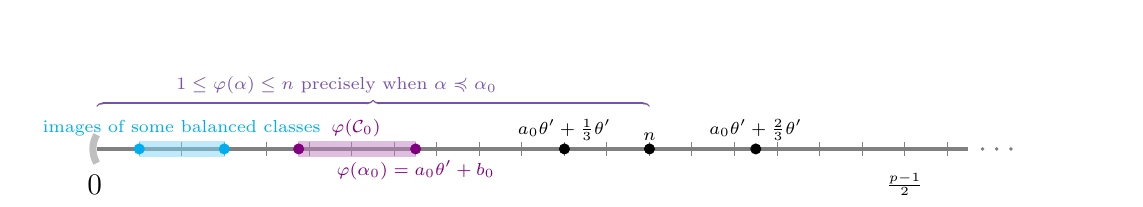
\begin{tikzpicture}
\scalebox{.9}{
\def \x {3/5}

\draw[gray, ultra thick] (0,4) -- (20.5*\x,4);  
\foreach \y in {1,...,20}
\draw[draw=gray] (\y*\x,4.1)--(\y*\x,3.9);
\draw[gray, line width=1mm, opacity=.5] (0,4.2) arc[start angle=150, end angle=210, radius=.4cm];
\node[left] at (.2,3.5) {{\large  $0$}};
\node at (19*\x,3.5) {{\scriptsize $\frac{p-1}{2}$}};
\filldraw[gray] (20.5*\x+0.2,4) circle (0.5pt);
\filldraw[gray] (20.5*\x+0.4,4) circle (0.5pt);
\filldraw[gray] (20.5*\x+0.6,4) circle (0.5pt);

%%% balanced class
\filldraw [cyan!50!white, opacity=0.5] (1*\x,4.1) rectangle (3*\x,3.9);
\node at (2*\x,4.3) {\textcolor{cyan}{{\scriptsize images of some balanced classes}}};
%
 \node[left] at (1*\x+.4,3.7) {};% {{\textcolor{cyan}{\scriptsize $m \theta$}}};
 \filldraw[cyan] (1*\x,4) circle (2pt);
% %
 \node[left] at (3*\x+.4,3.7) {};% {{\textcolor{cyan}{\scriptsize $M \theta$}}};
 \filldraw[cyan] (3*\x,4) circle (2pt);

%%% unbalanced class
 \filldraw [violet!50!white, opacity=0.5] (4.75*\x,4.1) rectangle (7.5*\x,3.9);
\node at (6.1*\x,4.3) {\textcolor{violet}{{\scriptsize $\varphi(\mathcal{C}_0)$}}};
%
 \node[left] at (4.75*\x+.4,3.7) {};% {{\textcolor{cyan}{\scriptsize $m \theta$}}};
 \filldraw[violet] (4.75*\x,4) circle (2pt);
% %
 \node at (7.5*\x,3.7) {{\textcolor{violet}{\scriptsize $\varphi(\alpha_0) = a_0\theta' + b_0$}}};
 \filldraw[violet] (7.5*\x,4) circle (2pt);

 %
\node[above] at (11*\x,4) {{\scriptsize $a_0 \theta' + \frac{1}{3}\theta'$}};
\filldraw[black] (11*\x,4) circle (2pt);
%

 %
\node[above] at (13*\x,4) {{\scriptsize $n$}};
\filldraw[black] (13*\x,4) circle (2pt);
%

 %
\node[above] at (15.5*\x,4) {{\scriptsize $a_0 \theta' + \frac{2}{3}\theta'$}};
\filldraw[black] (15.5*\x,4) circle (2pt);
%

 \draw [pen colour={royalpurple}, decorate, decoration = {calligraphic brace}, thick] (0,4.6) --  (13*\x,4.6);
 \node[right] at (1,4.9) {{\textcolor{royalpurple}{\scriptsize  $1 \leq \varphi(\alpha)  \leq n$ precisely when  $\alpha \preccurlyeq \alpha_0$}}};
}
\end{tikzpicture}
\caption{
Image of \(\varphi\) 
on \(\Z\) 
as well as  the positions of constants used in the proof of  \autoref{thm:quadratic} to determine that \(v_p(u_k)\neq 0\) for \(k\) that satisfy \(a_0\theta'+\frac{1}{3}\theta' \le k \le a_0\theta'+\frac{2}{3}\theta'\). 
Note that the preimages \(\alpha\in\mathcal{R}\) such that \(1\le \varphi(\alpha)\le n\) are precisely those roots for which~$\alpha \preccurlyeq \alpha_0$.}
\label{fig:pretty-things}
\end{figure*}


\subsection{Threshold conditions}
\label{subsec-thre}
Next we exhibit a threshold $B$ (defined in terms of the
recurrence~\eqref{eq:rel}) such that for all $n>B$ there are
rational integers $\theta'$ and $p$, with $p>n$ prime, satisfying the
following conditions:
\begin{enumerate}
\item[(P1)] $m_\theta(\theta')\equiv 0\pmod{p}$;
\item[(P2)]  The function $\varphi:\mathcal{R}\rightarrow\Z$ defined by
\[  \varphi(a\theta+b) = \begin{cases}
a\theta' + b & \text{if } a> 0,\\
a\theta' + b + p  & \text{if } a\leq 0
\end{cases}\]
is an order embedding of $(\mathcal{R},\prec)$
in $(\{0,1,\ldots,p-1\},<)$.
\item[(P3)] The set $\{ \alpha \in \mathcal{R} : 1 \leq \varphi(\alpha)
  \leq n \}$ is unbalanced.
\end{enumerate}

The definitions for $\theta'$ and $p$  follow.
Consider
the interval
\[ I(n):= \left\{ k\in\N : \frac{6n}{3a_0+2}\leq k-1\leq
    \frac{6n}{3a_0+1} \right\} \]    
    and let
$M:= \max\{a^2+|\beta|b^2 : a\theta+b \in \mathcal{R} \}$.  
By this choice $M$ is an upper bound of the norm of every element of $\mathcal R$.  By
\autoref{theo:bigprimespolyT}, there is an effective threshold~$B$ (which we may assume to be greater than $3M(M+1)$)
such that for all $n>B$ there exists a prime $p > 3Mn$ that divides the
product
\[ \prod_{\substack{k\in I(n)\\ k \in 2\N+1}} k^2-\beta.\]
Further, since \(p>3Mn\) is prime, we deduce that for \(n>B\) there exists 
$k_0 \in I(n) \cap (2\N+1)$ such that $k_0^2 \equiv \beta \pmod{p}$. 
We define $\theta' \in \N$ to be the number such that $k_0=2\theta'+1$.

We will show that $\theta'$ and $p$ satisfy Conditions (P1)--(P3).  Now
\begin{equation*}
    m_\theta(\theta') = m_\theta \biggl(\frac{k_0 - 1}{2} \biggr) \equiv k_0^2-\beta \equiv 0 \pmod{p}.
\end{equation*}
Thus $\theta'$ satisfies
Condition (P1).

We turn next to establishing Condition (P2).
Since $k_0\in I(n)$ and $k_0=2\theta'+1$, we have
\begin{equation}
(a_0+\textstyle\frac{1}{3})\theta' \leq n \leq
(a_0+\textstyle\frac{2}{3})\theta'.
  \label{eq:INEQ}
\end{equation}
Combining~\eqref{eq:INEQ} with the inequality $1\leq a_0 \leq M$ and rearranging terms gives 
$\frac{n}{M+1} \leq \theta' \leq \frac{3n}{4}$.
Recalling that $p>3Mn$ and $n > B \geq 3M(M+1)$, we conclude that
\begin{equation}
3M \leq \theta' \leq \frac{p}{4M} \, . 
\label{eq:INEQQ}
\end{equation}
The inequality $\theta'\leq\frac{p}{4M}$
in~\eqref{eq:INEQQ}
implies that for all roots \(a\theta + b \in \mathcal{R}\), $\varphi(a\theta+b)$ is equal to
    \begin{align*}
       a\theta' + b \in &
            \left\{0,\ldots,\frac{p-1}{2}\right\} \text{ if } a>0, \text{ and } \\
       a\theta' + b + p \in & \left\{\frac{p-1}{2},\ldots,p\right\} \text{ if } a\leq 0
    \end{align*}
(for the latter, recall that $\mathcal{R}$ contains no positive integers).  
Further, since have $|b| \leq M<\theta'$
for all $a\theta+b\in \mathcal{R}$, we conclude that
$\varphi$ is an order
embedding of $(\mathcal{R},\prec)$ into 
$(\{0,\ldots,p-1\},<)$.
This establishes (P2).

Equation~\eqref{eq:INEQ}  
and the inequality $\theta' > 3M$ from~\eqref{eq:INEQQ}
yields \[ \varphi(\alpha_0) < a_0\theta'+M < n < (a_0+1)\theta'-M \, .\] 
Hence \(\varphi(\alpha_0)\), the image of the greatest element in \(\mathcal{C}_0\) is upper bounded by \(n\).
From the definition of the order \((\mathcal{R},\preccurlyeq)\), for
$\alpha\in\mathcal R$ we have that $\alpha\preccurlyeq \alpha_0$ if and only if
$\varphi(\alpha) \leq n$.  
Thus (P3) follows from the fact that the set
$\{\alpha\in\mathcal{R}:\alpha \preccurlyeq \alpha_0\}$ is unbalanced.

\subsection{Prime divisors of \texorpdfstring{$u_n$}{un}}
\label{subsec-primediv}

To conclude the proof, we now explain why properties (P1)--(P3) imply that
$p$ divides $u_n$.  
Define $\psi:\Z[\theta]\rightarrow \Z/p\Z$ by
\[ \psi(a\theta+b):=(a\theta'+b)\bmod{p}.\]  
Condition (P2) entails that
$\psi$ and $\varphi$ agree on $\mathcal R$, while Condition (P1) entails
that~$\psi$ is a ring homomorphism. 
(We note in passing that the kernel of $\psi$ is a prime 
ideal~$\mathfrak{p}$ appearing in prime ideal factorisation of $p\Z[\theta]$.)
Hence the polynomial $fg$ splits
over $\Z/p\Z$ and $\varphi$ maps the roots of $fg$ in $\K$ to roots of
$fg$ in $\Z/p\Z$.  



Consider the decomposition of the \(p\)-adic valuation
\begin{equation*}
    v_p(u_n) = \sum_{k=1}^n (v_p(g(k))-v_p(f(k))).
\end{equation*}

Let $h(x)$ be an irreducible factor of either $f$ or $g$.
Then $h(x)$ is monic, of degree at most $2$ and height at most $M$.  Since $p>3Mn$, we easily see that $|h(k)|<p^2$
for all $1\leq k \leq n$ and hence
$v_p(h(k)) \in \{0,1\}$.
It follows that $v_p(u_n)$ is equal to the number of roots of $g$ 
in $\Z/p\Z$ that lie in $\{1,\ldots,n\}$ minus the number of roots of $f$ in $\Z/p\Z$ that lie in $\{1,\ldots,n\}$, counting repeated roots according to their multiplicity. 
Observe that this count takes place on the set \(\{\alpha\in\mathcal{R} : 1\le \varphi(\alpha)\le n\}\).
By Condition (P3), the aforementioned set is unbalanced and so it quickly follows that
$v_p(u_n)\neq 0$.

\subsection{Concluding the proof of \autoref{theo-decide-quad}}
\label{subsec-conclud}
Finally, let us return to the decidability of the Membership Problem in the setting of \autoref{theo-decide-quad}.
By our standing assumption that all instances of the problem are normalised we have that $t\neq 0$.  We have exhibited a bound $B$ such that for all $n>B$ there exists a prime $p>3Mn$
such that $v_p(u_n)\neq 0$.  This means that if $p_0$ is the largest prime such that $v_{p_0}(t)\neq 0$ then
for $n>\max\left(B,\frac{p_0}{3M}\right)$ we have $u_n\neq t$.
Thus we have reduced the Membership Problem in this setting to a finite search problem.
This immediately establishes decidability and concludes our proof of \autoref{theo-decide-quad}.


\section{Discussion} \label{sec:discussion}
In light of the results in~\Cref{sec-unequalsplitting}
a clear direction for further research is to 
examine the decidability of the Membership Problem for recurrences whose polynomial coefficients share the same splitting field.  
We recall that previous work \cite{NPSW022} established decidability when the polynomial coefficients split over the rationals.  The present work considers the case when the two polynomials split over the ring of integers of a quadratic field.  In future work we will consider the more general case in which the all roots of the coefficient polynomials have degree at most two. 
As far as the authors are aware, the only known results in this direction are the (un)conditional decidability results for quadratic parameters in~\cite{kenison2022applications}.
Extending the approach of the present paper to the case of polynomials with roots of degree more than two would require new results on large prime divisors on the values of such polynomials, which is an active area of research in number theory.

%\SkipTocEntry\section*{Acknowledgements}

\bibliographystyle{plain}
\bibliography{literature}

\appendix









\section{Proofs for Section~\ref{sec-polyseq}}
\label{sec:app-lowerbownun}

\begin{proof}[Proof of \autoref{claim:sizefunnyQ}]
First note that $A=\frac{b-a}{c}$.
The claim states that
\[ \log(F_n)	\geq \frac{2(b-a)}{c} (n\log n - n) \, .\]

The proof is as follows.
Given $y\in \N$, we first observe that 
\[\prod_{cx \leq y} (cx)^2 \geq   c^{2y}\bigg(\bigg\lfloor\frac{y}{c} \bigg\rfloor!\bigg)^2.\]
By Stirling's formula, the logarithm of the  quantity above is at least 
\begin{equation}
\label{eq:logQI}
\frac{2y}{c}\log c+ \frac{2y}{c} \log y -\frac{2y}{c}.
\end{equation}

Now \(F_n = \prod_{k\in I(n)} (k^2+\beta)\) is bounded from below by
\begin{equation*}
	F_n \geq \prod_{k\in I(n)} k^2
	\geq \prod_{ an\leq cx \leq bn} (cx+d)^2 
	\geq \prod_{ an\leq cx \leq bn} (cx)^2.
	\end{equation*}
By the above, and Equation~\eqref{eq:logQI} we conclude that \(\log(F_n)\) is bounded from below by
\begin{equation*}
	\log \prod_{cx \leq bn} c^2x^2  - \log \prod_{cx \leq an} c^2x^2
	\geq  \frac{2(b-a)}{c}( n \log n -n),
\end{equation*}
as required.  
\end{proof}

We now prove the inequality~\eqref{eq:BOUND} from the proof
of~\Cref{theo:bigprimespolyT}.
Noting that $A=\frac{b-a}{c}$, the inequality states
that
\begin{equation}
  e_p \leq  \frac{2An}{p-1}+  \frac{\varepsilon_2 \log n}{\log p}
\tag{\ref{eq:BOUND}}
\end{equation}

\begin{proof}[Proof of Inequality \eqref{eq:BOUND}]

If $e_p=0$ then the bound trivially holds.
Suppose $e_p>0$.  Then the function $f$ has two roots in $\Z/p\Z$.
Define $g\in\Z[x]$ by $g(x):=f(cx+d)$.
In case $p>c$ then $g$ also has two roots in $\Z/p\Z$.
For all $n\in\N$ define the products
\begin{equation*}
    G_n:=\prod_{k=1}^{\left\lfloor \frac{bn-d}{c} \right\rfloor} g(k)
    \quad \text{and} \quad
    H_n:=\prod_{k=1}^{\left\lceil \frac{an-d}{c} \right\rceil - 1} g(k)
\end{equation*}
    Then $F_n=\frac{G_n}{H_n}$ and hence
    $e_p=v_p(F_n)=v_p(G_n)-v_p(H_n)$.
Applying \Cref{prop:moll}, we get, for some constant $\varepsilon>0$,
\begin{align*}
v_p(G_n) \leq & \frac{2(bn-d)}{c(p-1)} + \frac{\varepsilon\log 
n}{\log p} \qquad {\text{ and }  }\\
v_p(H_n) \geq & \frac{2(an-d-c)}{c(p-1)} -
\frac{\varepsilon\log 
n}{\log p}.
\end{align*}
The upper bound in~\eqref{eq:BOUND} follows, for a suitable
choice of the constant $\varepsilon_2$, by subtracting the
upper bound for $v_p(G_n)$ from the lower bound for $v_p(H_n)$.
\end{proof}

\section{Second Case in the proof of Theorem~\ref{theo-decide-quad}}
\label{app-sec-quad}

Let $\beta \not\equiv 1 \pmod{4}$ be a square-free integer and
$\K=\Q(\sqrt{\beta})$ a quadratic field over which the polynomials $f$
and $g$ in~\eqref{eq:rel} split completely.  By Theorem~\ref{thm:quadratic}, the ring of integers of the field 
$\K$ is $\Z[\sqrt{\beta}]$. We define $\theta:=\sqrt{\beta}$,
so that $m_{\theta}:=x^2-\beta$ is the minimal polynomial of~$\theta$. 

Exactly as in Subsection~\ref{subsec-partition-roots}, we partition the set $\mathcal R$ of roots of $fg$ into classes, define the balanced and unbalanced classes, define the linear ordering~$\prec$ on $\mathcal R$, and consider the \emph{least unbalanced class} $C_0$.  
Let $a_0\theta+b_0$ be the greatest element in $C_0$ and note that $a_0\geq 1$ as before.


\subsection{Threshold conditions}
Next we exhibit a threshold $B$ (defined in terms of the
recurrence~\eqref{eq:rel}) such that for all $n>B$ there are
rational integers $\theta'$ and $p$, with $p>n$ prime, satisfying the three
conditions (P1)--(P3) as stated in Subsection~\ref{subsec-thre}.



The definitions for $\theta'$ and $p$ are as follows.
Consider
the interval
\[ I(n):= \left\{ k\in\N : \frac{3n}{3a_0+2}\leq k \leq
    \frac{3n}{3a_0+1} \right\} \] 
    and let
    $M$ be an upper bound on $\{|a|,|b|: a \theta+b\in 
\mathcal{R}\}$, and the height of the minimal polynomials of the elements of $\mathcal{R}$.
By
\autoref{theo:bigprimespolyT}, there is an effective threshold $B$, which we may assume to be greater than $3M(M+1)$,
such that for all $n>B$ there exists a prime $p > 3Mn$ that divides the
product
\[ \prod_{k\in I(n)} k^2-\beta.\]
Further, since \(p>3Mn\) is prime, we deduce that for \(n>B\) there exists 
$\theta' \in I(n)$ such that $(\theta')^2 \equiv \beta \pmod{p}$. 

We will show that $\theta'$ and $p$ satisfy Conditions (P1)--(P3).  Now
\begin{equation*}
    m_\theta(\theta') \equiv (\theta')^2-\beta \equiv 0 \pmod{p}.
\end{equation*}
Thus $\theta'$ satisfies
Condition (P1).

We turn next to establishing Condition (P2).
Since $\theta'\in I(n)$, it is straightforward to show that
\begin{equation}
(a_0+\textstyle\frac{1}{3})\theta' \leq n \leq
(a_0+\textstyle\frac{2}{3})\theta' \, .
  \label{app-eq:INEQ}
\end{equation}
These 
  bounds are identical to those in~\eqref{eq:INEQ}.
  In this case, Conditions (P2) and (P3) follow by an analogous argument to that given in Subsection~\ref{subsec-thre}.

\bigskip
\bigskip

The remaining part of the proof for the case $\beta\equiv  1 \pmod{4}$, as given  in Subsection~\ref{subsec-primediv} and Subsection~~\ref{subsec-conclud}, carries over to the present case without change. 


\end{document}